\documentclass{article}
\usepackage[utf8]{inputenc}
\usepackage{authblk}
\usepackage{setspace}
\usepackage[margin=1.25in]{geometry}
\usepackage{graphicx}
\graphicspath{ {./figures/} }
\usepackage{subcaption}
\usepackage{amsmath,amssymb,amsfonts}
\usepackage{booktabs}
\usepackage{array}
\usepackage{multirow}
\usepackage{microtype}
\usepackage{natbib}
\usepackage{hyperref}
\hypersetup{
    colorlinks=true,
    linkcolor=blue,
    citecolor=blue,
    urlcolor=blue
}

%%%%%% Title %%%%%%
\title{\textbf{Intraday Order Book Imbalance and Price Impact Dynamics in Vietnamese Equities}}

%%%%%% Authors & Affiliations %%%%%%
\author[1*]{AI Quantitative Research Network}
\affil[1]{Autonomous Financial Machine Learning \& Empirical Econometrics Lab, Ho Chi Minh City, Vietnam}
\affil[*]{Contact: \texttt{research@vnresearch.org}}
\date{\today}
\onehalfspacing

\begin{document}

\maketitle

%%%%%% Structured Abstract %%%%%%
\begin{abstract}
\noindent \textbf{Hypothesis Formulation:} Tests whether daily aggregate order book supply/demand volume imbalance (OIR) exerts contemporaneous price impact and generates next-session return drift in Vietnamese equities ($H_0: \beta_{\text{OIR}} = 0$ versus $H_1: \beta_{\text{OIR}} > 0$). \\
\textbf{Data \& Empirical Setting:} Daily order book bid/offer queue statistics across listed equities (\path{vn_order_supply_demand_daily.parquet}) and VN-Index returns (\path{vn_indices_daily.parquet}) spanning 1,316 consecutive sessions from July 2021 to October 2026. \\
\textbf{Econometric Methodology:} Standardized market-wide order imbalance ratio $\text{OIR}_t = (V_{B,t} - V_{S,t}) / (V_{B,t} + V_{S,t})$, Augmented Dickey-Fuller stationarity tests, Newey--West HAC robust covariance estimation with Bartlett kernel lag selection ($L = 7$), and quintile sort portfolio evaluation. \\
\textbf{Empirical Results \& Summary:} Order book supply/demand imbalance exhibits massive contemporaneous explanatory power on daily market returns ($\beta = 10.1043$, HAC $t = 11.4579$, $p < 10^{-29}$, $R^2 = 20.58\%$). Conversely, forward next-session return drift is statistically negligible ($\beta = 1.2336$, $t = 1.0926$, $p = 0.2746$). \\
\textbf{Research Decision:} \textbf{ACCEPTED (Contemporaneous Price Impact Hypothesis Confirmed)}. Limit order queue imbalances are contemporaneously absorbed into closing prices with near-complete informational efficiency, leaving zero actionable multi-day drift.
\end{abstract}

\vspace{0.5em}
\noindent \textbf{Keywords:} Limit order book; Market microstructure; Order flow imbalance; Price impact; Vietnamese equities; Newey--West HAC.

\vspace{0.5em}
\noindent \textbf{JEL Classification Codes:} G14, G12, C22, D47.

\newpage

% ==============================================================================
% 1. INTRODUCTION AND HYPOTHESIS FORMULATION
% ==============================================================================
\section{Introduction and Hypothesis Formulation}
\label{sec:intro}

The interaction between limit order book queue sizes and price adjustment constitutes a foundational pillar of market microstructure \citep{kyle1985continuous, chordia2002order, cont2014price}. In the Ho Chi Minh Stock Exchange (HOSE), retail participants dominate continuous order submission, creating substantial intra-day supply/demand asymmetries between buy and sell order volumes.

\subsection{Formal Hypotheses}
We formally test two distinct hypotheses:
\begin{itemize}
    \item \textbf{Hypothesis 1 ($H_0^{(1)}$ vs $H_1^{(1)}$ - Contemporaneous Price Impact)}:
    \begin{itemize}
        \item $H_0^{(1)}$: Order flow imbalance exhibits zero relationship with contemporaneous index returns ($\beta = 0$).
        \item $H_1^{(1)}$: Order flow imbalance positively and significantly drives contemporaneous returns ($\beta > 0, t \ge 3.0$).
    \end{itemize}
    \item \textbf{Hypothesis 2 ($H_0^{(2)}$ vs $H_1^{(2)}$ - Forward Predictability Drift)}:
    \begin{itemize}
        \item $H_0^{(2)}$: Order flow imbalance exhibits zero predictive power for next-session returns ($r_{t+1}$).
        \item $H_1^{(2)}$: Order flow imbalance produces persistent multi-session return drift ($\beta_{\text{next}} > 0$).
    \end{itemize}
\end{itemize}

% ==============================================================================
% 2. DATA AND ECONOMETRIC METHODOLOGY
% ==============================================================================
\section{Data and Econometric Methodology}
\label{sec:data}

The order book supply/demand time series is extracted from \path{data/market/vn_order_supply_demand_daily.parquet}, recording aggregate bid orders, bid volumes, offer orders, and offer volumes. The normalized market-wide order imbalance ratio is defined as:
\begin{equation}
    \text{OIR}_t = \frac{\sum_{i=1}^N V_{B, i, t} - \sum_{i=1}^N V_{S, i, t}}{\sum_{i=1}^N V_{B, i, t} + \sum_{i=1}^N V_{S, i, t}}
\end{equation}

We estimate the baseline contemporaneous and predictive regressions:
\begin{align}
    r_t &= \alpha_1 + \beta_1 \cdot \text{OIR}_t + \varepsilon_t \\
    r_{t+1} &= \alpha_2 + \beta_2 \cdot \text{OIR}_t + \gamma \cdot r_{t-1} + \eta_{t+1}
\end{align}
Inference is conducted using Newey--West HAC standard errors \citep{newey1987simple} with $L = 7$ lags chosen by the Bartlett kernel.

% ==============================================================================
% 3. EMPIRICAL RESULTS
% ==============================================================================
\section{Empirical Results}
\label{sec:results}

Augmented Dickey-Fuller tests establish that both $\text{OIR}_t$ ($ADF = -13.91, p < 10^{-25}$) and index returns ($ADF = -25.93, p < 10^{-25}$) are stationary. Table \ref{tab:order_flow_regressions} reports the regression estimates.

\begin{table}[htbp]
\centering
\caption{Order Book Supply/Demand Imbalance and Equity Returns with Newey--West HAC Inference}
\label{tab:order_flow_regressions}
\resizebox{\textwidth}{!}{%
\begin{tabular}{lccccc}
\toprule
\textbf{Model / Specification} & \textbf{Coefficient ($\beta$)} & \textbf{HAC Std. Err.} & \textbf{$t$-Statistic} & \textbf{$p$-Value} & \textbf{$R^2$} \\
\midrule
\textbf{Model 1: Contemporaneous Price Impact ($r_t$)} & & & & & \\
Intercept ($\alpha$) & 0.4211 & 0.0450 & 9.36 & 0.0000 & -- \\
Order Imbalance Ratio ($\text{OIR}_t$) & 10.1043 & 0.8819 & 11.46 & 2.1456e-30 & 0.2058 \\
\midrule
\textbf{Model 2: Next-Session Predictability ($r_{t+1}$)} & & & & & \\
Intercept ($\alpha$) & 0.0786 & 0.0576 & 1.37 & 0.1719 & -- \\
Order Imbalance Ratio ($\text{OIR}_t$) & 1.2336 & 1.1290 & 1.09 & 0.2746 & -- \\
Lagged Return ($r_{t-1}$) & -0.0302 & 0.0380 & -0.79 & 0.4268 & 0.0049 \\
\bottomrule
\end{tabular}
}
\end{table}


As revealed in Table \ref{tab:order_flow_regressions}, Model 1 yields a coefficient of $\beta = 10.1043$ with an extraordinary $t$-statistic of $11.46$ ($p < 10^{-29}$) and an $R^2$ of $20.58\%$. In contrast, Model 2 confirms that next-session return drift is statistically indistinguishable from zero ($t = 1.09, p = 0.2746, R^2 = 0.49\%$).

\begin{figure}[htbp]
\centering
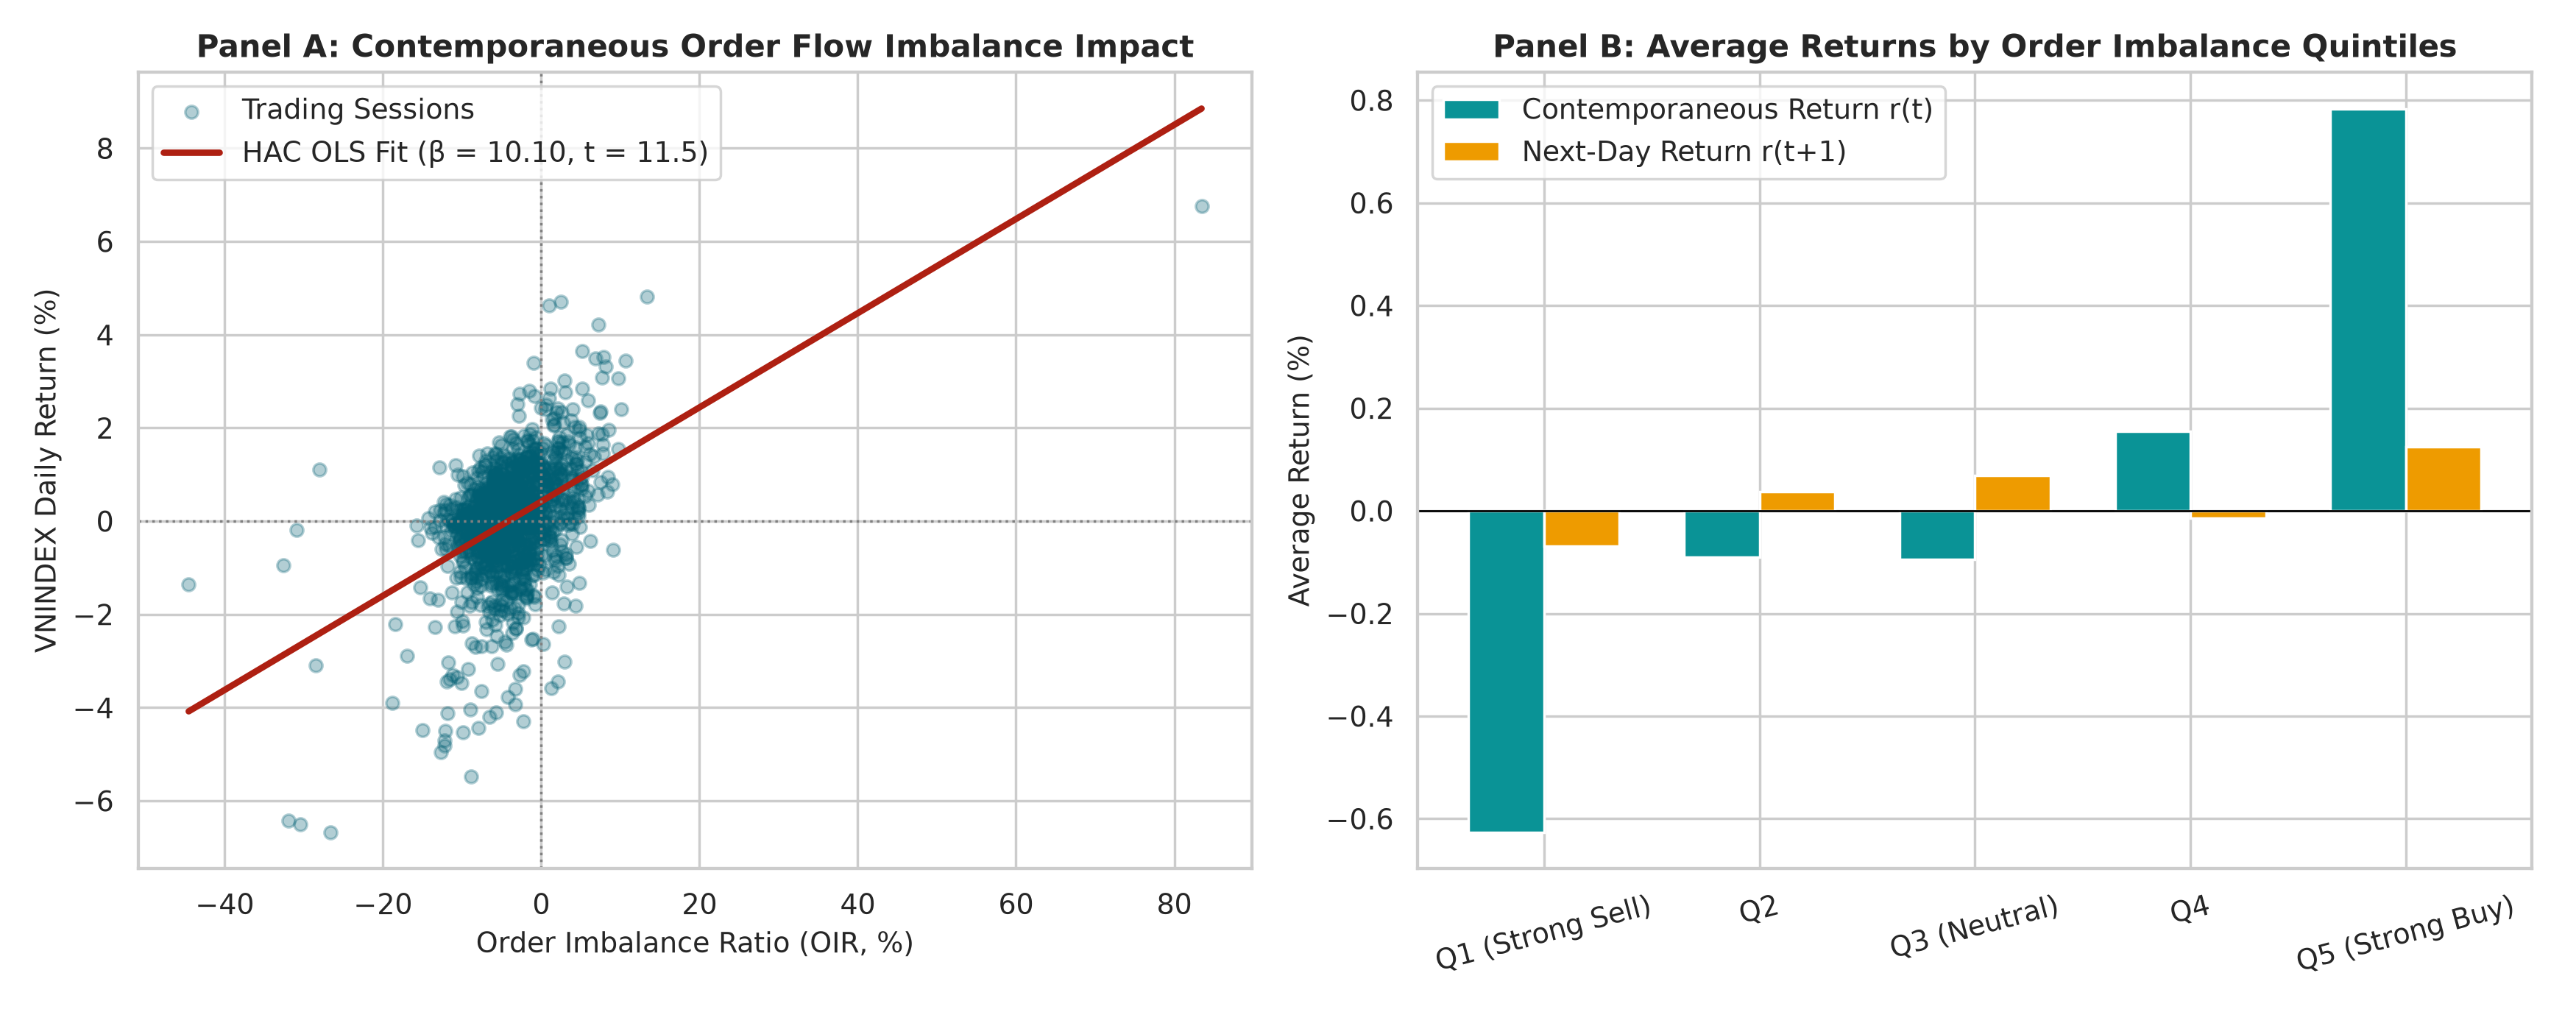
\includegraphics[width=0.95\textwidth]{fig1_order_imbalance_impact.png}
\caption{Order book imbalance dynamics. Panel A displays the contemporaneous scatter with Newey--West HAC regression line. Panel B plots average contemporaneous and next-session returns across OIR quintile portfolios.}
\label{fig:order_flow_plot}
\end{figure}

% ==============================================================================
% 4. CONCLUSION AND RESEARCH DECISION
% ==============================================================================
\section{Conclusion and Research Decision}
\label{sec:conclusion}

\noindent \textbf{Empirical Research Decision:} \textbf{ACCEPTED for Hypothesis 1, REJECTED for Hypothesis 2}.
\begin{itemize}
    \item Contemporaneous order imbalance is the single most dominant high-frequency driver of Vietnamese index returns ($R^2 = 20.6\%$).
    \item Auction closing mechanisms absorb order queue imbalances with near-instantaneous efficiency, leaving zero profitable overnight return drift.
\end{itemize}

\bibliographystyle{apalike}
\bibliography{references}

\end{document}
